\documentclass[a4paper]{report}

\newcommand\TBW{({\em to be written})}

\addtolength{\textwidth}{+1.5in}
\addtolength{\oddsidemargin}{-0.75in}
\addtolength{\evensidemargin}{-0.75in}
\addtolength{\textheight}{+1.5in}
\addtolength{\topmargin}{-0.75in}

\usepackage{amsmath}
\usepackage{amssymb}
\usepackage{multind}
\usepackage{url}
\usepackage{graphicx}
\usepackage{hyperref}
\usepackage{color}
\usepackage{txfonts}
\usepackage{prettyref}

\newcommand{\myimp}{\verb+ :- +}
\newcommand{\q}{\hspace*{1em}}
\newcommand{\algrule}{\noindent\rule{\textwidth}{0.1mm}}
\newcommand{\mysubsubsection}[1]{\subsubsection{$\diamond$ #1}}
\newcommand{\defined}{\stackrel{\mathrm{def}}{=}}
\newcommand{\bvec}[1]{\boldsymbol{#1}}
\newcommand{\vE}{\bvec{E}}
\newcommand{\valpha}{\alpha}
\newcommand{\kldiv}[2]{\mathrm{KL}(#1\;||\;#2)}
\newcommand{\argmax}{\operatornamewithlimits{argmax}}
\newcommand{\argmin}{\operatornamewithlimits{argmin}}
\newcommand{\noargs}{{\footnotesize [{\it no args}]\ }}

\newcommand{\conindex}[1]{\index{concept}{#1}}
\newcommand{\predindex}[1]{\index{predicate}{#1@{\tt #1}}}
\newcommand{\declindex}[1]{\index{predicate}{#1@{\tt #1} (declaration)}}
\newcommand{\optindex}[1]{\index{predicate}{#1@{\tt #1} ({\tt prism/2} option)}}
\newcommand{\flagindex}[1]{\index{predicate}{#1@{\tt #1} (execution flag)}}
\newcommand{\statindex}[1]{\index{predicate}{#1@{\tt #1} (statistic)}}
\newcommand{\commindex}[1]{\index{predicate}{#1@{\tt #1} (system command/file)}}
\newcommand{\envindex}[1]{\index{predicate}{#1@{\tt #1} (environment variable)}}
\newcommand{\bpindex}[1]{\index{predicate}{#1@{\tt #1} (B-Prolog built-in)}}
\newcommand{\distindex}[1]{\index{predicate}{#1@{\tt #1} (built-in distribution)}}
\newcommand{\pcindex}[1]{\index{predicate}{#1@{\tt #1} (built-in pseudo counts)}}
\newcommand{\exindex}[1]{\index{example}{#1}}
\newcommand{\progindex}[1]{\index{example}{#1@{\tt #1}}}
\newcommand{\secref}[1]{\S\ref{#1}}
\newcommand{\tablestart}{\mathit{table\_start}}
\newcommand{\memo}{\mathit{memo}}
\newcommand{\chkcmpl}{\mathit{check\_complete}}
\newcommand{\lb}{\linebreak[3]}
\newcommand{\data}{\bvec{G}}
\newcommand{\Hburn}{H_{\mbox{\footnotesize burn-in}}}
\newcommand{\Hskip}{H_{\mbox{\footnotesize skip}}}

\newcommand{\vlambda}{\lambda}
\newcommand{\vtheta}{\theta}
\newcommand{\va}{a}
\newcommand{\vd}{d}
\newcommand{\vx}{x}
\newcommand{\vy}{y}
\newcommand{\qdb}{q}
\newcommand{\db}{\mathit{DB}}
\newcommand{\weight}{w}

%%% 2.3
\newcommand{\vw}{\bvec{w}}
\newcommand{\vB}{\bvec{B}}
\newcommand{\vG}{\bvec{G}}
%%%
\newcommand{\mvec}[1]{\mathbf{#1}}
\newcommand{\mset}[1]{\mathbf{#1}}
\newcommand{\mmat}[1]{\mathbf{#1}}
%\newcommand{\argmax}{\mathop{\rm argmax}\limits}
%\newcommand{\argmin}{\mathop{\rm argmin}\limits}
\newcommand{\commentsize}{\footnotesize}
\newcommand{\Pre}{\mathbf{\rm Pre}}
\newcommand{\sitepath}[1]{{\sf #1}}
\newcommand{\action}[1]{{\tt #1}}
\newcommand{\nonterminal}[1]{{\sf #1}}
\newcommand{\method}[1]{{\sf #1}}

\newcommand{\defeq}{\ensuremath{\stackrel{\mathrm{def}}{=}}}

%\newcommand{\db}{\mathit{DB}}
\newcommand{\pdb}{P_\mathit{DB}}
\newcommand{\msw}{\mbox{\tt msw}}
\newcommand{\tensor}{\mbox{\tt tensor}}
\newcommand{\indexfunc}{T}
\newcommand{\einsum}{\mbox{einsum}}
\newcommand{\minx}{\mbox{min}_1}

\bibliographystyle{plain}
\makeindex{concept}
\makeindex{predicate}
\makeindex{example}

\newrefformat{chap}{Chapter \ref{#1}}
\begin{document}
	\begin{center}
		\par\vspace*{3cm}\par
		%{\Huge\bf PRISM User's Manual}\par\vspace*{0.5cm}\par
		{\Huge\bf T-PRISM User's Manual}\par\vspace*{0.5cm}\par
		{\Large }\par\vspace*{12cm}\par
		
		%{\normalsize Taisuke Sato, Neng-Fa Zhou, Yoshitaka Kameya, Yusuke Izumi, Keiichi Kubota and Ryosuke Kojima}
		
		%{\normalsize * Tokyo Institute of Technology} \\
		%{\normalsize \dag CUNY Brooklyn College} \\
		%{\normalsize \ddag Meijo University}
		
		\par\vspace*{2cm}\par
		
		%{\footnotesize Copyright \copyright~2017 T. Sato, N.-F. Zhou, Y. Kameya, Y. Izumi, K. Kubota and R. Kojima}
	\end{center}
	\thispagestyle{empty}
	\setcounter{page}{0}%% quick hack for hyperref
	\clearpage
	
	
	\pagenumbering{roman}
\section*{Preface}

PRISM is a declarative probabilistic logic programming language which can perform efficient probability calculation by probabilistic propositional calculation based on distribution semantics.
On the other hand, deep learning frameworks such as Tensorflow attracts attention in recent years with the development of deep learning techniques.
Also, by using these frameworks, it is easy to calculate multidimensional array (tensor) including high-speed matrix calculation using GPGPU.
That is why that introducing calculation using Tensorflow and deep learning techniques to PRISM is expected to improve the current PRISM system.


\section*{Installation}
The following packages are required to compile T-PRISM system.
\begin{itemize}
	\item protobuf   $\geq$ 3.0
	\item libhdf5    
	\item Python     $\geq$ 3.7
	\item tensorflow $\geq$ 1.10.0
\end{itemize}

In Ubuntu 18.04 or later, you can prepare the protobuf and libhdf5 by the following procedure.
\begin{verbatim}
$ apt-get install -y libhdf5-dev libprotobuf-dev protobuf-compiler 
\end{verbatim}

To install Python3.7, we recommend using Anaconda, a Python platform for data science.
First, the install script for Anaconda can be download as follows: 
\begin{verbatim}
$ curl -O https://repo.anaconda.com/archive/Anaconda3-2019.03-Linux-x86_64.sh
\end{verbatim}

Then, you can execute the downloaded scripts and follow the instructions. In many cases, default settings and yes answers are suitable (see the official page for details: \url{https://www.anaconda.com/})

\begin{verbatim}
$ sh Anaconda3-2019.03-Linux-x86_64.sh
\end{verbatim}

After installing Python, tensorflow is required to install as the following commands according to your environment:
\begin{itemize}
	\item tensorflow (with CPU) for python3
	\begin{verbatim}
$ pip install tensorflow
	\end{verbatim}
	\item  tensorflow (with GPU) for python3
	\begin{verbatim}
$ pip install tensorflow-gpu
	\end{verbatim}
\end{itemize}


\subsection*{Manual install: protobuf}
If you use Ubuntu 16.04 or earlier, the version of protobuf by using the default package manager (apt-get) is less than 3.0; hence, manual installation of protobuf $\geq$ 3.0 is required.
This section describes the brief instruction for manual installation (see the official page for details: \url{https://developers.google.com/protocol-buffers/}).

First, you can download and install {\tt protobuf-all-3.5.1.tar.gz} by the following commands:
\begin{verbatim}
$ wget https://github.com/google/protobuf/releases/download/v3.5.1/protobuf-all-3.5.1.tar.gz
$ tar xvf protobuf-all-3.5.1.tar.gz
$ cd protobuf-3.5.1
$ ./autogen.sh

$ ./configure
$ make
$ make check
$ sudo make install
$ sudo ldconfig
\end{verbatim}

Then, let us install the protobuf for python by the following commands:
\begin{verbatim}
$ cd python/
$ CFLAGS=-std=c++11 python3 setup.py build --cpp_implementation
$ CFLAGS=-std=c++11 python3 setup.py install --cpp_implementation
\end{verbatim}

\subsection*{Docker image}
A pre-build docker image for the latest PRSIM including T-PRISM is provided in the Dockerhub (\url{https://hub.docker.com/r/prismplp/prism}). 
If you have docker-installed machines, you can use our pre-built docker image  as the following command:

\begin{verbatim}
docker pull prismplp/prism
\end{verbatim}

\chapter{T-PRISM}
\label{chap:tprism_semantics}




\section{Tensorized least model semantics}

T-PRISM's   semantics,  ``tensorized   least   model  semantics''   or
``tensorized semantics'' for short,  is a tensorized generalization of
the  distribution semantics  \cite{Sato95}, i.e.,  the existing  PRISM
semantics.  In  PRISM, the  semantics  assigns  probability masses  to
ground atoms  in the Herbrand base  for a program whereas  in T-PRISM,
tensors containing real values are assigned to them.
%Probability measure over the Herbrand interpretations of DB.
We first describe formally a class of primitive programs of T-PRISM to
explain the  tensorized semantics,  and then describe  actual programs
and implementation.

Formally,   a   primitive   program    is   a   quadruple   $\left\langle
F,C,T,q_F\right\rangle$. A primary part of the program $\db=F \cup C $
is a pure Prolog (definite clause) program  where $F$ is a set of {\em
	tensor atom\/}s  (see below),  and $C$  is a  set of  definite clauses
whose head contains no tensor  atom. Theoretically, we always equate a
set of clauses  with the set of all ground  instances, and allow $\db$
to be countably infinite.

In addition to this  setting, we introduce a set of  tensors $T$ and a
specific type of atoms called  {\em tensor atom\/}s having a predicate
name  {\tt  tensor/2}  to  identify  a  tensor  called  {\em  embedded
	tensor\/} in $T$.  A  tensor atom also has an {\em  index\/} as a list
of Prolog  constants at the second  argument to access entries  of the
identified tensor.   For example  ${\tt tensor(x,[i,j])}$ is  a tensor
atom  having a  ground  atom {\tt  x}  and an  index  {\tt [i,j]}.  It
declares a  second-order tensor  (matrix) specified  by {\tt  x} whose
index $(i,j)$ is expressed by {\tt [i,j]}. To make this correspondence
rigorous,  we define  a  function $q_F(\cdot)$  from  tensor atoms  to
embedded  tensors such  that  $q_F({\tt tensor(x,[i,j])})=x_{ij}$.  In
general,  an  index  of  an  $n$-order tensor  is  represented  as  an
$n$-length  list  of  Prolog  constants. When  a  tensor  atom  occurs
multiple times  in a  program, different  indices may  be used  in the
program to access its entries,  for example, {\tt tensor(x,[i,j])} and
{\tt  tensor(x,[k,l])} may  occur in  the program  to access  the same
embedded tensor {\tt x}.  To specify the size of an embedded tensor, a
special  predicate {\tt  tensor\_atom/2}  is used.  For example,  {\tt
	tensor\_atom(x,[20,20])}  means  that  a  $20  \times  20$  matrix  is
associated with all tensor atoms like {\tt tensor(x,\_)}.

In  this paper,  as already  shown, we  use italic  fonts for  indices
appearing  in mathematical  expressions to  distinguish them  from the
corresponding ones appearing  in a program. So for  a matrix specified
by {\tt x}, we write an entry $x_{ij}$ for the index {\tt [i,j]}.

%So we
%define a mapping $I_F$ from an atom {\tt x} to a set of all possible
%indices of the embedded tensor $\mmat{X}$ specified by {\tt x} in the
%program. For example, when we define $I_F({\tt x})= \{(i,j),
%(k,l)\}$, 
%By using
%$I_F(\cdot)$ and $R(\cdot)$, the dimensional consistency of tensors
%such as $K_i = K_k$ and $K_j = K_l$ can be checked.

%Although we have been dealing with vectors (one-dimensional arrays) so
%far, without loss of generality, it is straightforward to handle
%multi-dimensional arrays by replacing an index with a tuple of
%indices.
%For example, a matrix $\mmat{X}_{ij}$ associated with a
%tensor $\tensor_x$ is introduced by
%$q_F(\tensor(x,[i,j]))= \mmat{X}_{ij}$ and
%$\indexfunc_F(\tensor(x,[i,j]))=(i,j)$. 

Once a T-PRISM program is given, a set of {\it tensor equation\/}s are
determined from the program. Consider a  clause having a head $H$. Let
$H  \leftarrow  W_{\ell}  (\ell  =1,\ldots,L)$ be  an  enumeration  of
clauses   about  $H$   in   the  program.   For   each  $H$,   logical
equations\footnote{
	%
	Logical equivalence seems a more appropriate term, but we use equation
	for intuitiveness.
	%
} of the following form are derived that hold in the least model of
the program.
%
\begin{align} \nonumber
H &\Leftrightarrow W_{1} \vee W_{2} \vee ... \vee W_{L} \\
W_{\ell} &\defeq B_{1\ell} \wedge B_{2\ell} \wedge ... \wedge B_{M_\ell \ell}
\label{eq:logic_eqs}
\end{align}
%
where $B_{*\ell}$ is a ground atom in the body $W_{\ell}$.

The  tensorized  semantics  is   obtained  by  expanding  the  mapping
$q_F(\cdot)$ over $F$  to $q(\cdot)$ for the entire  Herbrand base. It
assigns various orders  of tensors to atoms as  their denotation. They
are inductively defined,  starting from tensor atoms,  by applying two
rules below to \prettyref{eq:logic_eqs}.
%As condition, we introduce the following constraint:
%$\indexfunc(W_{1})=\indexfunc(W_{2})=...=\indexfunc(W_{L})$.
%Under this condition, the following two rules related to embedded values and indices associated with each ground atom are introduced.
\begin{description}
	\item [Disjunction rule]
	Given a disjunction of tensor atoms, its embedding
	is defined as the summation of the tensor atoms, $A$ and $B$:
	%
	\[q(A \vee B) \defeq q(A)+ q(B).\]
	% Here$\indexfunc(A_{a} \vee A_{b}) = \indexfunc(A_{a}) = \indexfunc(A_{b})$ is assumed.
	%This rule say that an embedding of a disjunction consisting of vector-embedded atoms is a vector.
	%When embedded values are multi-dimensional array, .
	%Applying this rule to the \prettyref{eq:t_prism_eqs},
	%$\indexfunc(H)=\indexfunc(W_{1})=\indexfunc(W_{2})=...=\indexfunc(W_{L})$
	%is derived.
	%while
	%assuming the condition
	%$\indexfunc(W_{1})=\indexfunc(W_{2})=...=\indexfunc(W_{L})$ named {\it
	%disjunction pre-condition}
	%As condition, we introduce the following constraint:
	%$\indexfunc(W_{1})=\indexfunc(W_{2})=...=\indexfunc(W_{L})$.
	\item [Conjunction rule]
	Given a conjunction of tensor atoms with associated multi-dimensional
	arrays for embedding, embeddings of the conjunction is defined by the
	{\em Einstein's notation\/} rule\footnote{
		%
		Although a general formulation of Einstein's notation distinguishes
		between covariance and contravariance, indicated by subscript and
		superscript indices respectively, their distinction is irrelevant to
		our semantics, and hence ignored in this paper.
		%
	}.  In the case where subscripts overlap in the same term, the rule is
	to take a sum for that subscript. We call the overlapping index a {\em
		dummy  index\/}  whereas  a  non-overlapping  index  as  a  {\em  free
		index\/}. A  set of free indices  is assigned to the  whole term. When
	the index is  empty, the resulting value is a  scalar (number) and the
	value of  a conjunction of  scalar embedding  atoms is the  product of
	their values.
	
	%For example, put $\indexfunc(A)=(i,j)$ and
	%$\indexfunc(B)=(j,k)$. $\indexfunc(A \wedge B)=(i,k)$ is computed by
	%this rule, and a matrix is embedded to $q(A \wedge B)$. As a result,
	%its $i,k$-th element $q(A \wedge B)_{ik}$ is computed as $\sum_j
	%q(A)_{ij} \cdot q(B)_{jk}$, i.e., this computation coincides with
	%matrix multiplication.
\end{description}
%
By applying  these rules  to \prettyref{eq:logic_eqs}  recursively, we
can derive a  set of tensor equations, and the  working sample program
in \prettyref{sec:distmult01} is written with the definitions introduced
so far.

For more flexible modeling  and concise descriptions, T-PRISM introduces
also the following concepts and conventions:

\begin{description}
	\item [Tensor subgoal]
	An index  of the ground  atoms except  for tensor atoms  is implicitly
	determined  by  the above  rules.  When  the  same ground  atoms  with
	different   indices  occur   multiple  times   however,  an   explicit
	description is  required.  We  introduce a  meta description  for such
	explicit  index   specification  ${\tt  subgoal(g,[i,j])}$   which  is
	interpreted  logically as  ${\tt subgoal(g,  [i, j])}  \Leftrightarrow
	{\tt g}$ but  implementationally as $q({\tt subgoal(g,[i,j])})=g_{ij}$
	for numerical calculation.  This process can be  regarded as rewriting
	the free indices not bounded by the clause.
	
	\item [Non-linear operation]
	Non-linear  operations   are  prerequisites   for  a  wide   range  of
	applications including  deep neural networks. To  make them available,
	T-PRISM provides  {\tt operator/1} indicating a  non-linear operation,
	e.g.,  {\tt operator(sigmoid)}  represents  a  sigmoid function.  This
	built-in predicate occurs in the equation similarly to {\tt tensor/2}.
	For example, let $A$ and $B$  be tensor atoms. $B \Leftrightarrow {\tt
		operator}(f)  \wedge {\tt  operator}(g)  \wedge A$  is interpreted  as
	$q(B) = f(g(q(A))) = f \circ  g (q(A))$ where $\circ$ represents their
	function    synthesis.    While    ${\tt    operator}(f)\wedge    {\tt
		operator}(g)   \wedge    A$   and   ${\tt    operator}(g)\wedge   {\tt
		operator}(f) \wedge A$ are  logically equivalent, they are interpreted
	as different equations: $f(g(q(A)))$ and $g(f(q(A)))$, respectively.
	
	\item [Non-tensor fact and predicate] 
	Although the above formulation does not include (non-tensorized) facts
	in the  logic programming,  a fact  can be regarded  as a  tensor atom
	assigned one (a scalar value) like existing PRISM.  Furthermore, a
	non-tensor  predicate, which  does not  contain any  tensor atom  like
	Prolog standard built-in predicates, also  can be regarded as having a
	scalar value one assignment like  PRISM. In the actual implementation,
	these  predicates are  proved by  Prolog engine  and omitted  from the
	equation (see the next section ).
\end{description}

By applying these rules to \prettyref{eq:logic_eqs} recursively, we
can derive the following tensor equations:
%
\begin{align}\nonumber
q(H) & = q(W_1) + q(W_2) + ... + q(W_{L}) \\ \nonumber
q(W_{\ell}) & = op_1 \circ op_2 \circ ... \circ op_{O_k} \\
& \circ \einsum_{q,T}(q(B_{1\ell}), q(B_{2\ell}) ... q(B_{M'_\ell \ell}))
\label{eq:tprism_eqs}
\end{align}
%
where $\einsum_{q,T}$ is a sum-product operation indicated by the
Einstein's notation, $op_1, op_2, ..., op_{O_k}$ are non-linear
operations, $\{B_{1\ell}, B_{2\ell},\ldots, B_{M'_\ell \ell}\}$ are
ground atoms except for {\tt operator/1}, including tensor atoms. We
consider the derived set of tensor equations as the {\em formal
	denotation\/} of the given T-PRISM program in the tensorized
semantics.
%has a least solution (as all coefficients are
%non-negative)\cite{sato2017linear} and
In this paper, we assume \prettyref{eq:tprism_eqs} is well-defined,
i.e., there is no mismatch of tensor dimensions.


%% fact is one
%% non tensor predicates including prolog standard built-in predicates

\section{Concepts in T-PRISM}
\label{sec:concepts}
Theoretically T-PRISM is an implementation of the tensorized semantics with a specific execution mechanism.
%The main idea of T-PRISM program execution is that the symbolic part of program execution including
%recursion is processed by Prolog search and the numerical and parallel
%part such as loop for sum-product computation is carried out by
%TensorFlow. The division of labor is interfaced by explanation graphs.
This section describes the technical issues on implementation and application of T-PRISM.

\subsection*{Tensorized explanation graphs}
\label{pre}
More  concretely  in  T-PRISM,  a  program is  first  compiled  to  an
explanation   graph   representing   a  set   of   logical   equations
like   \prettyref{eq:logic_eqs}.  Next,   the  explanation   graph  is
translated      to      a       set      of      tensor      equations
like  \prettyref{eq:tprism_eqs}. By  converting  the tensor  equations
into a  TensorFlow program, the  parameter training and  inference are
carried out efficiently by parallelization. This section details these
compilation steps.

Let $G$ be a top goal.  The first step for generating tensor equations
is  to  construct  an  explanation graph  by  exhaustive  search  that
represents the  set of  all proof trees  for $G$ as  a set  of logical
equations.  To efficiently  calculate  this set,  T-PRISM adopts  {\em
	tabled search\/} in  the exhaustive search for all  proofs and applies
dynamic  programming  to them.  The  tabled  search is  a  memoization
technique specialized for Prolog  search \cite{Zhou08}.  It stores the
results of successful  calls of a goal and returns  the stored answers
when  the same  goal  occurs  later again.   When  all predicates  are
selected for  tabling, the resulting  set of tensor  equations exactly
corresponds to  the set of  logical equations representing  all proofs
for $G$ in \prettyref{eq:tprism_eqs}.  We  call it the {\em tensorized
	explanation  graph\/} for  $G$.   By  removing redundant  repetitions,
Einstein's notation  enables sum-product computation much  faster than
that in PRISM.  Hereafter, we simply call it explanation graph.

We here remark on an  optional assumption on explanation graphs called
the {\it  acyclic condition\/}  \cite{Sato08a}.  When  the explanation
graph is cyclic,  it is converted to a set  of recursive equations and
T-PRISM can compute  its least fixed point by  iteratively solving the
set of equations.  Note that various efficient inference and parameter
training   algorithms    are   available   for    cyclic   explanation
graphs \cite{sato2014infinite,kojimaprefix} and it is shown that cycle
explanation   graphs  bring   about   flexible   modeling  of   cyclic
relations \cite{kojima2015goal} in PRISM.
%This paper describes a sample program using a cyclic explanation graph for transitive closure in the section 4.
Although this  paper does  not treat  cyclic explanation  graphs, such
extension    of   T-PRISM    would    simulate   interesting    models
like \cite{sato2017linear}.


%To formally state it, we introduce a binary relation $G^{(\ell)} \succ
%G_{n}$ over defined goals such that $G^{(\ell)} \succ G_{n}$ holds if
%$G^{(\ell)}$ is the head of some defining formula and $G_{n}$ occurs
%in the body. When ``$\succ$'' is acyclic in ${\rm expl}(G)$, ${\rm
%	expl}(G)$ is said to be {\it acyclic\/} and we extend ``$\succ$'' to a
%partial ordering over the defined atoms. Explanation graphs which are
%not acyclic are called cyclic. Once an acyclic ${\rm expl}(G)$ is
%constructed, minimal atoms in the partial ordering ``$\succ$'' have
%only tensor atoms in the body of their defining formula whose
%embeddings and the assigned indices are declared in the program. So we
%can compute indices for defined atoms from the bottom layer consisting
%of minimal atoms upward in a dynamic programming manner in time linear
%in the size of ${\rm expl}(G)$, i.e., the number of atoms appearing in
%${\rm expl}(G)$. Also, by the same bottom-up manner, $q(G^{(\ell)})$
%is computed by applying sum-product operations to all defined goals.
%%

\subsection*{Parameter training}

To train parameters in embedded tensors, T-PRISM supports (stochastic)
gradient  decent algorithms  using an  auto-differential mechanism  in
TensorFlow.  We compute the loss of a dataset $D$ represented as a set
of  goals to  learn parameters.   T-PRISM  assumes the  total loss  is
defined   to    be   the    sum   of    individual   goal    loss   as
follows:
\begin{equation}
Loss(D)=\sum_{G \in D} Loss(G).
\end{equation}

Usually, $Loss(G)$ is a function of $q(G)$. For example, when
parameter training uses a negative log likelihood loss function, the
goal loss function is defined as $Loss(G)=-\log q(G)$
where $q(G)$ stands for the likelihood of $G$.
For the convenience of modeling, the T-PRISM system offers related
built-ins for parameter training and custom loss functions written by
Python programs with TensorFlow.
A loss function can be specified as a runtime argument for parameter training.
Utilizing this T-PRISM system based on tensorized semantics with non-linear operators,
various models including matrix computation, deep neural networks, and the models written by recursive programs can be designed.


Here is the case of supervised learning in which $G$ is represented as
$goal(y,x)$ where $x$ is an input data and $y$ is a label.

\begin{equation}
Loss(goal(y,x))=loss(y,q(goal(\_,x)))
\label{eq:loss_supervision}
\end{equation}
%%
where $\_$ is a dummy variable and $loss$ is a loss function such as
cross-entropy loss and mean square loss, where the first argument is a
correct output and the second argument is an output of the model. For
the convenience of modeling, the T-PRISM system offers related
built-ins for parameter training and custom loss functions written by
Python programs with TensorFlow. A loss function can be specified as
a runtime argument for parameter training.

\subsection*{Batched explanation graphs}
\label{sec:batched_eg}

The  minibatch  method  is  essential   in  deep  learning  and  other
optimization  problems  from  the  viewpoint  of  learning  speed  and
performance    \cite{Goodfellow-et-al-2016}.      A    straightforward
implementation thereof uses subgraphs of an explanation graph, and the
current     PRISM    system     adopts     this    naive     minibatch
method \cite{kojima2018ijar}.  However it  can further be optimized by
simultaneously conducting computations  on multiple explanation graphs
with isomorphic structure in a minibatch.

To help  the calculation  by isomorphic structure  in a  minibatch, we
introduce  {\em  batched explanation  graph\/}s,  where  the size  and
structure of explanation graphs in  a minibatch is common, independent
on  inputs.   We  use  a   meta  variable  for  inputs,   called  {\em
	placeholder}.  For  example, suppose  the proof trees  are constructed
for  {\tt  goal(P)},  where  {\tt  P}  is  a  dummy  variable.   After
constructing an  explanation graph,  actual terms are  substituted for
the dummy variable. The important thing here is that this substitution
preserves   the  explanation   graph   in  size   and  structure   and
parallelization  is made  possible by  adopting a  batched explanation
graph and converting it to computational graphs using the placeholders
in TensorFlow.

%For example,

%\section{The whole T-PRISM system}
%Given a top-goal, we search for all SLD proofs by tabled search.
\subsection*{Simulating PRISM}

Suppose the embedded tensors are scalar. Then it is possible to define
categorical  distributions using  $q_F(\cdot)$ and  some of  T-PRISM's
operations.   So  the  tensorized  semantics can  simulate  the  PRISM
semantics where  the disjunction rule  is reduced to the  summation of
probability  of exclusive  events  under the  exclusive assumption  in
PRISM \cite{Sato08a} and the conjunction rule is reduced to product of
probabilities of independent events.
%the marginalization of hidden variables where a dummy index is
%regarded as a hidden variable whose range equals that of the index.
Hence, the new semantics can be  considered as a generalization of the
distribution semantics. Although we cannot expect such a simulation to
be sped  up by  parallelization because of  scalar calculation,  it is
sometimes useful to  be able to construct a  T-PRISM program including
PRISM parts.
Concrete method to implementation of simulating PRISM is described in \prettyref{sec:simulated_msw}.

\chapter{T-PRISM system}

\begin{figure}[tb]
	\centering
	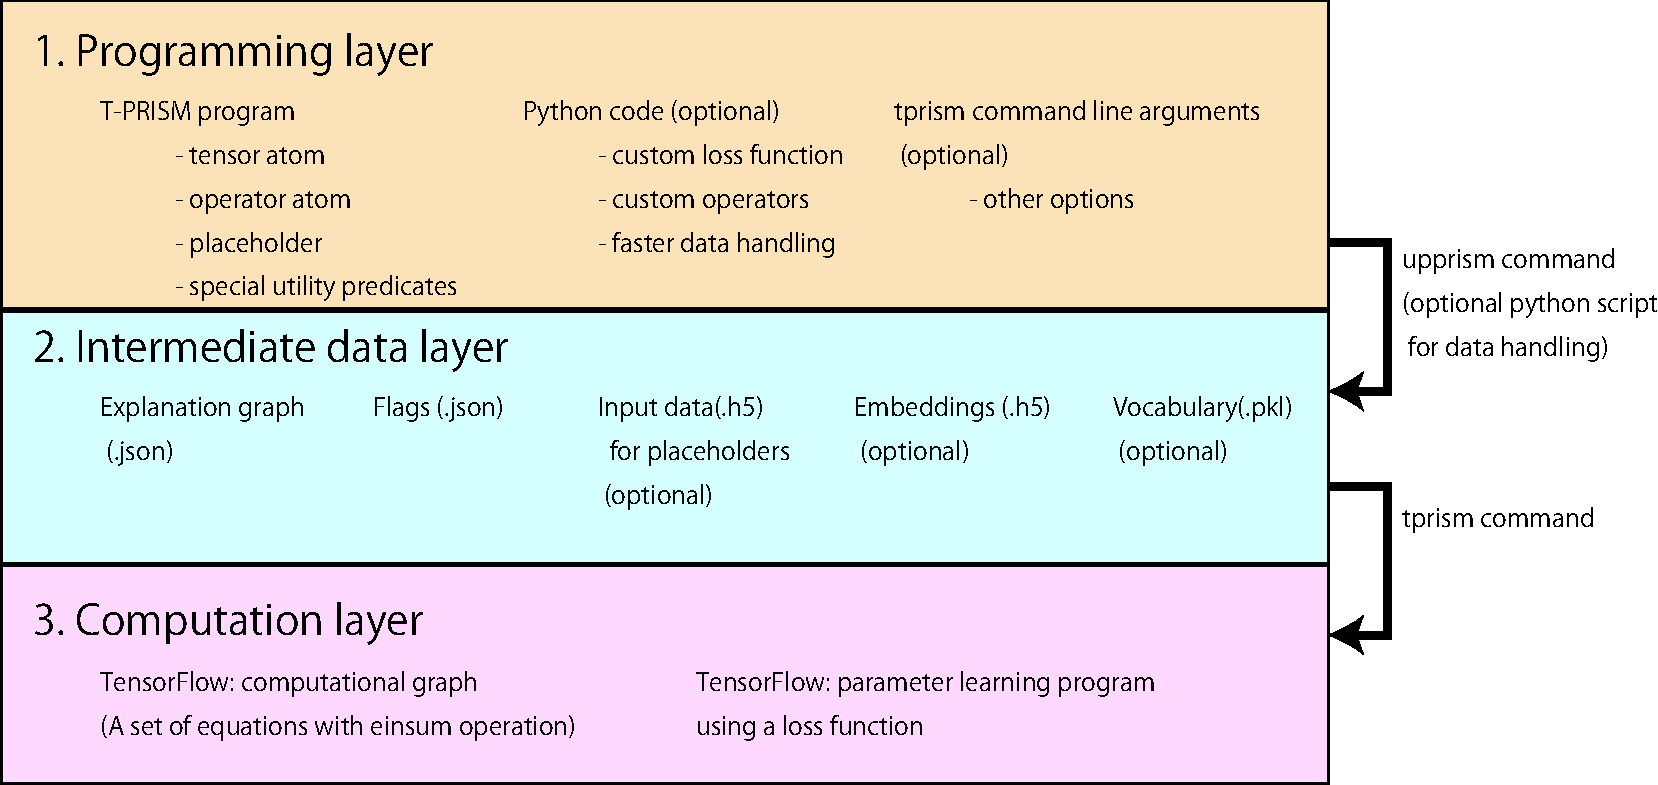
\includegraphics[width=1.0\linewidth]{tprism_system.pdf}
%	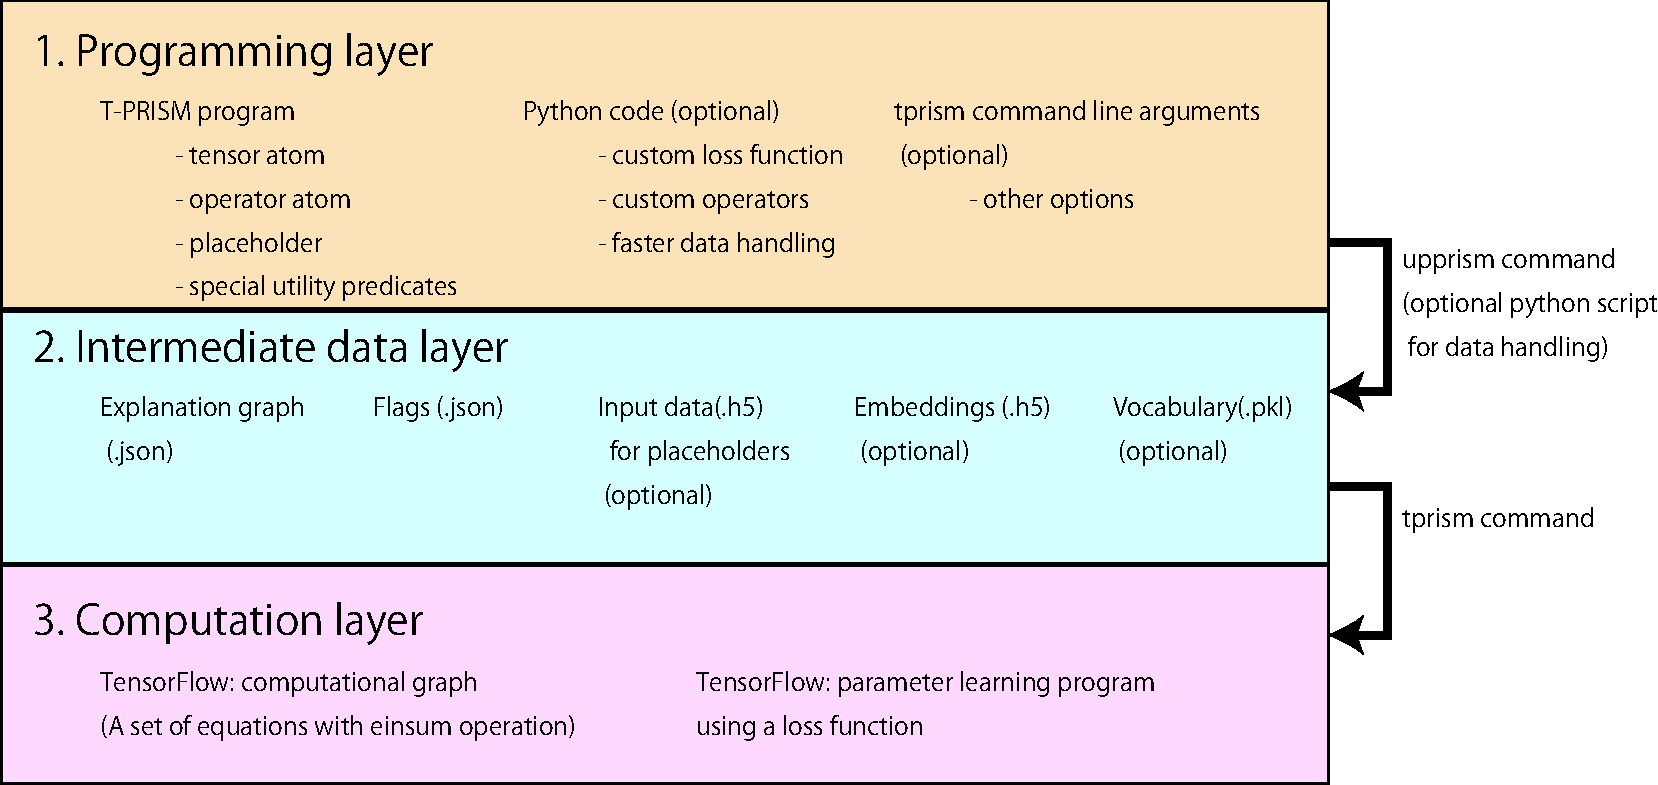
\includegraphics{tprism_system.pdf}
	\caption[T-PRISM system]{T-PRISM system}
	\label{fig:tprismsystem}
\end{figure}


The architecture of the T-PRISM system is shown in \prettyref{fig:tprismsystem}.
The T-PRISM system consists of three layers: programming layer, intermediate data layer, and calculation layer.

Although users directly operate the programming layer, they should understand the entire flow.
First, a T-PRISM program is converted into intermediate data using the {\it upprism} command, a command for batch execution of a PRISM program
(see the PRISM manual for details of upprism).
Then, learning and probability calculation is performed from the intermediate data using the {\it tprism} command, a special command for T-PRISM.
In a standard procedure consisting of training and test phases, the commands are executed in the following order.


\begin{verbatim}
$ upprism <tprism program>
$ tprism train <internal data options> <other options>
$ tprism test <internal data options> <other options>
\end{verbatim}
\verb|<tprism program>|, \verb|<internal data options>|, and \verb|<other options>| need to be properly replaced according to each case.
Usage of the tprism command is explained in \prettyref{sec:tprism_command}.



The programming layer contains three elements: T-PRISM program, Python code, tprism command-line argument.
The T-PRISM programs are written by combining Prolog programs and extended features such as tensor atoms, operator atoms, and placeholders by the following chapter (\prettyref{chap:tprism_semantics}).
In addition to these functions, T-PRISM system provides utility predicates for generating intermediate data.
These special predicates are described in \prettyref{sec:tprism_predicate}.

Next, Python codes of the programming layer are mainly used to define operations corresponding to user-defined loss function and operator atoms.
For these definitions, it is necessary to define the class according to the prescribed format and place the Python source codes in a predetermined place (those are placed in {\tt prism/bin/tprism/loss} for the custom loss functions, and the custom operations are placed in {\tt prism/bin/tprism/op}).
Python scripts also can be used for data handling.
Although it is possible to generate intermediate data with the T-PRISM program,
some utility predicates implemented in Prolog; therefore, Python scripts provides faster data handling.
In particular, since a generation of input data is often a simple conversion of data formats, Script languages like Python are suitable for data processing.
Concrete examples are shown in \prettyref{chap:tprism_sample}.


After the generation of intermediate data has been completed, learning and calculation can be performed from the intermediate data using the tprism command.
When executing the command, you can specify command-line arguments as \verb|<options>| in the above example to  set parameters for learning and calculation.
Some parameters can also be set using flags of the T-PRISM program.
If they are specified at the same time, the arguments take precedence over the flags.
Details of flags added for T-PRISM are described in \prettyref{sec:tprism_predicate}.

The intermediate data layer contains the following five files:
\begin{description}
	\item[Explanation graph] generated from a T-PRISM program is stored in a JSON file or a protocol buffer file.
	\item[Flags] specified in a T-PRISM program are stored in a JSON file or a protocol buffer file.
	\item[Input data] for placeholders is stored in an HDF5 file.
	\item[Embeddings] for tensor atoms and their embedded tensors are stored in an HDF5 file
	\item[Vocabulary] to associate a tensor atom with a multidimensional array is stored in a file. This file is automatically generated by tprism command at the time of training.
\end{description}
To save intermediate data, JSON (extension: .json) is mainly for structured data, and HDF5 (extension: .h5) format is mainly used for multidimensional array data.
A backend engine to save JSON files is the google protocol buffer; hence, these data can be saved as a protocol buffer format, and the protocol buffer engine provides the interface for the other programming languages.


\section{Special utilities in T-PRISM programs}
\label{sec:tprism_predicate}

In addition to PRISM's utilities, T-PRISM includes special utilities for passing data to the intermediate data layer.

\subsection*{Transport an explanation graph and flags from programming layer to intermediets layer}

The following predicates save the explanation graph constructed from a goal list {\it Goals}
as {\it ExplFilename}(default:expl.json) with {\it ExplMode} format (default:json) and the flags as {\it FlagFilename} (default:flag.json) with {\it FlagMode} format (default:json).
\begin{itemize}
	\item {\tt save\_expl\_graph}
	\item {\tt save\_expl\_graph({\it Goals})}
	\item {\tt save\_expl\_graph({\it ExplFilename},{\it FlagFilename})}
	\item {\tt save\_expl\_graph({\it ExplFilename},{\it FlagFilename},{\it Goals})}
	\item {\tt save\_expl\_graph({\it ExplFilename},{\it FlagFilename},{\it ExplMode},{\it FlagMode},{\it Goals})}
\end{itemize}
where this system supports {\tt json}, {\tt pb} (protocol buffer binary file), and {\tt pbtxt}(protocol buffer text file) as {\it ExplMode} and {\it FlagMode}.

Using these predicates, for example, the following description saves the explanation graph as {\tt sample.expl.json} and the flags as {\tt sample.flag.json}
by using {\tt save\_expl\_graph} with a goal list {\tt Gs}, restored from  {\tt sample.dat}.
\begin{verbatim}
prism_main([]):-
  load_clauses('sample.dat',Gs),
  save_expl_graph('sample.expl.json','sample.flag.json',Gs).
\end{verbatim}


The following predicates only save the current state of flags as a file name {\it FlagFilename} with {\it FlagMode} format(default: json).
\begin{itemize}
	\item {\tt save\_flags({\it FlagFilename})}
	\item {\tt save\_flags({\it FlagFilename},{\it FlagMode})}
\end{itemize}
Since these predicates only save the flag, goals are not required.


When executing with the upprism command, for example, the following description should be added to a T-PRISM program in addition to the model description.
\begin{verbatim}
prism_main([]):-save_flags('sample.flags.json').
\end{verbatim}


\subsection*{Handling placeholders and their substitution values}


The batched explanation graph described in \prettyref{sec:concepts} is an efficient method to handle isomorphic explanation graphs built independently of inputs.
The concrete example is shown in \prettyref{sec:distmult02} and \prettyref{sec:nn}.

To use placeholder, we need to separate a template of explanation graphs, i.e., a explanation graph containing placeholders, from input data, and then construct a correspondence table of the placeholders in as an input data file. 
Now, special predicates to save the correspondence table are described.
The following predicates use pattern matching between a goal and a pattern to determine a placeholder and its substitution value.
More concretely, the following predicates find a matched goal and a pattern from the ground goal list {\it Goals} and a list of patterns {\it PlaceholderGoals} including variables; therefore,
a pair of a variable and its substitution value is regarded as a placeholder and its realized value and saved as {\it Filename} (default: data.h5) with {\it Mode} format (default: h5fs).

\begin{itemize}
	\item {\tt save\_placeholder\_goals({\it PlaceholderGoals},{\it Goals})}
	\item {\tt save\_placeholder\_goals({\it Filename},{\it PlaceholderGoals},{\it Goals})}
	\item {\tt save\_placeholder\_goals({\it Filename},{\it Mode},{\it PlaceholderGoals},{\it Goals})}
\end{itemize}

For example, the following program constructs a placeholder in the form of pred/1 and its substitution values are (1,2,3,5,8).
\begin{verbatim}
prism_main([]):-
  Goals=[pred(1),pred(2),pred(3),pred(5),pred(8)],
  PlaceholderGoals=[pred(_)],
  save_placeholder_goals('data.h5',PlaceholderGoals,Goals).
\end{verbatim}
where information related to placeholder is saved in {\tt data.h5}.
Note that only the integer values are possible for the realization values of a placeholder in the current version T-PRISM system.

Now, let me consider another example.
The following program saves an explanation graph with placeholders using {\it PlaceholderGoals}
because {\tt save\_placeholder\_goal/3} predicate yields unification of all variables in {\it PlaceholderGoals} with special atom, or {\it placeholder atom}, to represent a placeholder.
Suppose that the goals are matched with a pattern{\tt rel(\_,\_)} in this example.
\begin{verbatim}
prism_main([]):-
  Goals=[rel(0,1),rel(1,2),rel(2,3)],
  PlaceholderGoals=[rel(_,_)],
  save_placeholder_goals('data.h5',PlaceholderGoals,Goals),
  save_expl_graph('sample.expl.json','sample.flag.json',PlaceholderGoals).
\end{verbatim}

In this case, \verb|PlaceholderGoals = [rel($placeholder1$,$placeholder2$)]| holds.
This is because in this system, placeholder atoms \verb|$placeholder1$, $placeholder2$, ...| are automatically assigned and unified to variables in order of appearance.
Information related to placeholders are saved in {\tt data.h5}, i.e., 
\verb|$placeholder1$| is associated with (0,1,2), and \verb|$placeholder2$| is associated with (1,2,3).

Finally, we describe lower-level predicates for creating an Input data file, i.e.,
predicates that directly stores a list of placeholders and their data as {\it Filename}.
\begin{itemize}
	\item {\tt save\_placeholder\_data({\it Placeholders},{\it Data})}
	\item {\tt save\_placeholder\_data({\it Filename},{\it Placeholders},{\it Data})}
	\item {\tt save\_placeholder\_data({\it Filename},{\it Mode},{\it Placeholders},{\it Data})}
\end{itemize}

{\it Placeholders} is a list of placeholders associated with each goal.
Let {\it Goals} be \verb|[pred(1),pred(2),pred(3),pred(5),pred(8)]|
and {\it PlaceholderGoals} be \verb|[pred(_)]|.
{\tt save\_placeholder\_goals({\it PlaceholderGoals},{\it Goals})}
 corresponds to {\tt save\_placeholder\_data({\it Placeholders},{\it Data})} with
{\it Placeholder}={\tt [[\$placeholder1\$]]} and {\it Data}={\tt [[[1],[2],[3],[5],[8]]]}.

We consider a more complex example containing two predicates: {\tt pred1} and {\tt pred2}.
\begin{verbatim}
prism_main([]):-
  Goals=[pred1(1,4),pred1(2,3),pred1(3,2),pred2(5,1),pred2(8,0)],
  PlaceholderGoals=[pred1(_,_),pred2(_,_)],
  save_placeholder_goals('data.h5',PlaceholderGoals,Goals).
\end{verbatim}
In this case, \verb|PlaceholderGoals| = \verb|[pred1($placeholder1$,$placeholder2$),pred2($placeholder3$,$placeholder4$)]| holds.
The relationship between placeholder atoms and associated vectors is as follows:

\begin{tabular}{|c|c|}
	\hline 
	placeholder atom& vector \\ 
	\hline 
	\verb|$placeholder1$|& $(1,2,3)$ \\ 
	\hline 
	\verb|$placeholder1$|& $(4,3,2)$ \\ 
	\hline 
	\verb|$placeholder1$|& $(5,8)$ \\ 
	\hline 
	\verb|$placeholder1$|& $(1,0)$ \\ 
	\hline 
\end{tabular} 

Using the low-level predicate, the same placeholders can be created by {\tt save\_placeholder\_data({\it Placeholders},{\it Data})} with
{\it Placeholder}={\tt [[\$placeholder1\$,\$placeholder2\$],[\$placeholder3\$,\$placeholder4\$]]}
and {\it Data} = {\tt [[[1,4],[2,3],[3,2]],[[5,1],[8,0]]]}.






\subsection{Special flags}
In the T-PRISM system, parameters and behaviors of learning and calculation are controlled using the tprism command.
Also, those can be controlled from the T-PRISM program using flags to control learning and calculation.

The way of handling flags is the same with PRISM, i.e, {\tt set\_prism\_flag} and {\tt get\_prism\_flag} are available.


A list of additional flags in the T-PRISM system is shown below.
\begin{itemize}
\item \verb|sgd_minibatch_size|(range: integer) determines the number of data in a minibatch for minibatch training.
\item \verb|epoch| or \verb|max_iterate|(range: integer) determines the maximum number of epochs for training.
\item \verb|sgd_learning_rate|(range: real value) determines the learning rate for the stochastic gradient decent method.
\end{itemize}


\section{tprism command}
\label{sec:tprism_command}

This section explains the tprism command, a command to read files in the intermediate data layer and to perform learning and calculation.
The tprism command is executed in the following format.
\begin{verbatim}
tprism <mode> [options...]
\end{verbatim}
For \verb|<mode>|, either train or test should be specified.
The options are as follows:
\begin{itemize}
	\item \verb|--intermediate_data_prefix|
specifies a directory where intermediate files, except for input data and embeddings files, are placed or a prefix of paths of intermediate files.
	For example, if you specify {\tt abc/}, it is equivalent to specifying the following options:
	\begin{verbatim}
		  --expl_graph abc/expl.json
		  --flags abc/flags.h5
		  --model abc/model.ckpt
		  --vocab abc/vocab.pkl
	\end{verbatim}
\end{itemize}

Intermediate  data
\begin{itemize}
	\item \verb|--expl_graph | specifies an explanation graph file name in intermediate data layer.	
	\item \verb|--flags | specifies a flags file name in intermediate data layer.	
	\item \verb|--model | specifies a file name of the model saved in the training phase and loaded in the test phase.
	\item \verb|--vocab | specifies a vocabulary file name in intermediate data layer.
	If the specified file does not exist, it is automatically generated at the time of learning.
\end{itemize}

Additional intermediate data
\begin{itemize}
	\item \verb|--embedding | specifies an embeddings file name in intermediate data layer.
	\item \verb|--data | specifies an input data file name in intermediate data layer.	
\end{itemize}

Learning
\begin{itemize}
	\item \verb|--sgd_loss| specifies a loss function. The name loss function allow built-in loss function: 
	\begin{description}
		\item [nll] negative log likelihood
		\item [ce] cross-entropy loss function
		\item [preference\_pair] a loss for preference learning
		the other custom loss function.
	\end{description}
	\item \verb|--cycle|: this option is added to solve equations including cycles. The details are described in \prettyref{sec:transitive_closure01}.
	\item \verb|--output | specifies a destination file of the prediction in the test phase. Currently, this command supports  numpy format, readable in Python.
\end{itemize}

Also, flag settings can be changed with options with the same name as flags.
\begin{itemize}
	\item \verb|--sgd_minibatch_size| 
	\item \verb|epoch| or \verb|--max_iterate|
	\item \verb|--sgd_learning_rate|
\end{itemize}

The other options:
\begin{itemize}
	\item \verb|--gpu GPU (default: all) (e.g. --gpu 0,2)|
	specifies GPU numbers to use.
	\item \verb|--cpu|
	this option disables GPU, and only CPUs are used.
	\item \verb|--no_verb| suppresses the message in the train and test phases.
\end{itemize}






\section{Intermediate data format}
\label{sec:intermediate_data}

This section describes the data format of the intermediate data.
Usually, the beginners do not directly refer to intermediate data.
It is also possible to perform data handling efficiently by directly operating with Python script or the other scripts.

\subsection{Explanation graph / Flags files}
The protocol buffer files to define data structure is written in 
\verb|prism/src/c/external/expl.proto|.

\subsection{Input data file}

An H5FS file, a general-purpose format, contains multiple {\it Groups}.
Named {\it datasets} can be stored for each Group, and dataset can include {\it attributes} and a {\it value}, which allows a multidimensional array as a value.

An input data file has groups corresponds to goal\_id, an identifier of a goal.
Dataset named as "data" contains a list of placeholders as an attribute
and their associated integer matrix ($\#$data $\times$  $\#$placeholders) as  a value.
Then, for example, an input data file can be read by the following Python script: 
\begin{verbatim}
import h5py

with h5py.File("data.h5", 'r') as f:
  for goal_id in f:
    print("goal_id:",goal_id)
    print("placeholders:",f[goal_id]["data"].attrs.get("placeholders"))
    print("data size:",f[goal_id]["data"].value.shape)
\end{verbatim}

The output of this program execution is as follows:
\begin{verbatim}
goal_id: 0
placeholders: [b'$placeholder1$' b'$placeholder2$']
data size: (100, 2)
\end{verbatim}


\subsection{Embedding file}

An embedding file contains two groups: "train" and "test".
Each group has datasets named as \verb|"tensor\_<tensor atom name>\_"|, and a dataset in this file is associated with a multidimensional array as its value.
\verb|<tensor atom name>| corresponds to a name of a tensor atom in a T-PRISM program.


Please refer to the example in MNIST below as an example of the program to generate this file.
\begin{verbatim}
prism/exs/tensor/mnist/build_dataset.py
\end{verbatim}

The ways to associate a tensor atom with a tensor are provided as the following cases:
\begin{itemize}
 \item Special tensor atoms: {\tt onehot/1}
 \item Embedding files generated by {\tt save\_embedding\_from\_pattern}
 \item Embedding files generated by Python scripts 
 \item The other tensor atoms are associated with randomly initialized tensors regarded as trainable parameters.
\end{itemize}

Specific names of tensor atoms are associated with fixed vectors.
The current version of T-PRISM supports one-hot encoding {\tt onehot/1}.
{\tt tensor\_atom(onehot(X),[Y])} is associated with a Y-dimension vector whose X-th element is one and the other elements are zero.
For example,
{\tt tensor\_atom(onehot(0),[3])} is associated with a vector (1,0,0),
and {\tt tensor\_atom(onehot(1),[5])} is associated with a vector (0,1,0,0,0).
Sample programs using {\tt onehot/1} are shown in \prettyref{sec:markov_chain} and \prettyref{sec:simulated_msw}.

The continued two ways are related to an embedding file.
An embedding file in intermediate data layer can be generated by {\tt save\_embedding\_from\_pattern}.
{\tt save\_embedding\_from\_pattern({\it Vars},{\it Pattern},{\it Target},{\it FileNameBase})}
constructs a fixed binary matrix, whose axes corresponds to {\it Vars}, from facts with a specific pattern {\it Pattern}. Furthermore, the constructed matrix is associated with a target tensor atom {\it Target} and this information is stored in {\it FileNameBase}.h5 and {\it FileNameBase}.csv files.
Note that the matrix size is automatically determined from pattern.
The example and details are described in \prettyref{sec:transitive_closure01}.
Another way to create embedding files is using Python scripts.
The sample is shown in \prettyref{sec:transitive_closure02}.



\chapter{Sample programs}
\label{chap:tprism_sample}

This chapter explains sample programs of T-PRISM:
\begin{enumerate}
\item Knowledge graph modeling using DistMult  \cite{Yang15}
\item An efficient implementation of DistMult
\item A recursive program for a  finite-state discrete-time  Markov chain
\item Transitive closure computation with cyclic explanation graphs
\item An efficient implementation of transitive closure computation
\item Learning a simple neural network with the MNIST dataset \cite{lecun1998mnist} for image recognition
\item Simulating PRISM and implement PCFG with T-PRISM
\end{enumerate}
These sample programs are available in \verb|exs/tensor| in the PRISM directory.

\section{Sample programs for knowledge graph modeling}
\label{sec:distmult01}

This sample program is available in \verb|prism/exs/tensor/distmult_sample01|.
Please also see README.md in this directory that explain how to run  this program.
This section describes the essential ideas and background of this scripts. 

\subsection*{Modeling}

\begin{figure}[tb]
	\begin{minipage}{0.5\hsize}
		%\rule{24em}{0.10mm}\\[0.6em]
		\rule{0.85\textwidth}{0.10mm}\\ [-1em]
		\begin{verbatim}
		1: tensor_atom(v(_),[20]).
		2: tensor_atom(r(_),[20]).
		3:
		4: rel(S,R,O):-
		5:   tensor(v(S),[i]),
		6:   tensor(v(O),[i]),
		7:   tensor(r(R),[i]).
		\end{verbatim}
		\rule{0.85\textwidth}{0.10mm}\\ [-1em]
		\caption{DistMult program in T-PRISM}
		\label{fig:tprism-distmult}
	\end{minipage}
	\begin{minipage}{0.5\hsize}
		%\rule{24em}{0.10mm}\\[0.6em]
		\rule{0.85\textwidth}{0.10mm}\\ [-1em]
		\begin{verbatim}
		1: values(v(_),[1-20]).
		2: values(r(_),[1,0]).
		3: 
		4: rel(S,R,O):-   %R=rel(S,O) in {0,1}
		5:   msw(v(S),C), %P(C_S=C|S)
		6:   msw(v(O),C), %P(C_O=C|O)
		7:   msw(r(C),R). %P(R=1|C_O=C,C_S=C)
		\end{verbatim}
		\rule{0.85\textwidth}{0.10mm}\\ [-1em]
		\caption{DistMult-like program in PRISM}
		\label{fig:prism-distmult}
	\end{minipage}
\end{figure}



We  first look  at  a  T-PRISM program  used  for  link prediction  in
knowledge  graphs.  A  knowledge graph  consists of  triples (subject,
relation, object) in the resource description framework (RDF).  Notice
that a  triple (subject, relation,  object) says that the  subject and
object  stand  in  the  ``relation'' and  this  fact  is  equivalently
represented  by a  ground atom  {\tt rel}(subject,  relation, object),
using the {\tt  rel}/3 predicate.  So logically  speaking, a knowledge
graph is nothing but a set of ground atoms.

For  link   prediction  in   knowledge  graphs,  we   choose  DistMult
model \cite{Yang15}, one  of the standard knowledge  graph models, for
its simplicity.  In DistMult, entities $s$, $o$, $r$ ($s$ for subject,
$o$ for  object, $r$ for  relation) are encoded as  N-dimensional real
vectors, $\mvec{s}$, $\mvec{o}$, and  $\mvec{r}$ respectively, and the
prediction is made based on the score of $(s,r,o)$ computed by:
%
\begin{equation}
f(s,r,o)=\sum_i \mvec{s}_i \mvec{r}_i \mvec{o}_i.
\label{eq:distmult}
\end{equation}

In      T-PRISM,      a       DistMult      model      is      written
like   \prettyref{fig:tprism-distmult}.     The   lines   1    and   2
introduce \verb|v(_)| and \verb|r(_)|.  They are embedded vectors with
an index  \verb|i|. The lines  3 says the  range of index  \verb|i| is
$0  \leq $\verb|i|$<  20$.  The  lines 5-8  represent an  equation for
sum-product computation  for the  three embedded vectors  required for
computing DistMult scores in \prettyref{eq:distmult}.



For  comparison, we  show  a PRISM  program  for DistMult-like  model
(PRISM-DistMult)
in \prettyref{fig:prism-distmult} \cite{kojima2018ijar}.  It encodes a
probabilistic binary  relation over pairs  of entities: a  subject $S$
and an object $O$ and the probability of $r(s,o)$ is computed by:
%P(C_S=i|S=s)P(C_O=i|O=o)P(R=1|C_O=i,C_S=i).
\begin{align}\nonumber
f'(s,r,o)=\sum_i & P(C_S=i \mid S=s) \\ \nonumber
&\hspace{1em} P(C_O=i \mid O=o) \\
&\hspace{1em} P(R=1 \mid C_O=i, C_S=i).
\label{eq:prism-distmult}
\end{align}
%
We can clearly see the isomorphism between this sum-product computation and the
one computed by the T-PRISM program in
\prettyref{fig:tprism-distmult}.
Both programs carry out essentially the same computation. However, the
current PRISM constructs redundant explanation graphs by expanding $i$
to  multiple  ground  atoms  with  arguments  varying  from  1  to  20
(specified  by  {\tt values(v(\_),[1-20])}),  due  to  the lack  of  a
collective sum-product operation specified by the Einstein's notation.
T-PRISM removes  this redundant construction of  explanation graphs in
terms of  the meta-variable $i$,  resulting in not only  memory saving
but  faster sum-product  operations.  Exploiting  this notation  and a
mechanism of batched explanation graphs described before makes T-PRISM
applicable to large scale applications.



For our link prediction experiment, we employ a loss function based on
negative log likelihood for the knowledge graph as follows:
%
\[Loss(rel(S,R,O)) = \left[ f(S, R, O) - f(S, R, O') -\gamma \right]_{+}\]
%
where $[\cdot]_{+}$ means  a hinge loss $max(0,\cdot)$  and a negative
sample  $O'$ is  uniformly sampled  from all  entities.  We  use this
hinge  loss  function  with   $L2$  regularization  and  its  learning
parameters set to $\lambda=1.0e-5$ and $\gamma=1$.


\subsection*{Program execution}
A sample program \verb|distmult_sample.psm| consists of a Distmult model like \prettyref{fig:tprism-distmult}, utility functions, and a batch script as follows: 
\begin{figure}[h]
	%\rule{24em}{0.10mm}\\[0.6em]
	\rule{0.85\textwidth}{0.10mm}\\ [-1em]
\begin{verbatim}
 1: prism_main([]):-
 2:   random_set_seed(1234),
 3:   load_clauses('sample.dat',Gs),
 4:   generate_preference_pair(Gs,GoalPairList),
 5:   save_expl_graph('distmult_sample_tmp/expl.json',
 6:                   'distmult_sample_tmp/flags.json',
 7:                   GoalPairList).
\end{verbatim}
\rule{0.85\textwidth}{0.10mm}\\ [-1em]
\end{figure}
This \verb|prism_main| is called using upprism command and save an explanation graph constructed from sample.dat.
A predicate \verb|generate_preference_pair| in this script performs sampling negative data at random to compute the loss function.
Finally, \verb|save_expl_graph/3| store the explanation graph and flags in \verb|distmult_sample_tmp/|.

By executing the following commands using this program, learning parameters and computation of link score using {\tt sample.dat} can be performed.
\begin{enumerate}
\item the following command constructs an explanation graph using {\tt sample.dat} and model written in {\tt distmult\_sample.psm} and saves it in \verb|distmult_sample_tmp/| with the other intermediate data.
\begin{verbatim}
$ cd prism/exs/tensor/
$ upprism distmult_sample.psm
\end{verbatim}
	
\item The following tprism command trains the parameter (tensors associated with tensor atoms) using a loss function {\tt preference\_pair} using the intermediate data in {\tt distmult\_sample}.
\begin{verbatim}
$ tprism train --intermediate_data_prefix distmult_sample_tmp/ --sgd_loss preference_pair
\end{verbatim}

\item The following tprism command computes a predictive loss using the trained model and the intermediate data in {\tt distmult\_sample\_tmp}.
\begin{verbatim}
$ tprism test --intermediate_data_prefix distmult_sample_tmp/ --sgd_loss preference_pair
\end{verbatim}
Note that this case does not split train and test datasets for simplicity.
To split a dataset into train and test datasets, intermediate data for train and test phases should be prepared.
\end{enumerate}



\section{An efficient implementation of DistMult}
\label{sec:distmult02}

This sample program is available in \verb|prism/exs/tensor/distmult_sample02|.
Please also see README.md in this directory that explain how to run  this program.
This section describes the essential ideas and background of this scripts. 


Let us consider the explanation graph used in the previous section.
Like PRISM, {\tt probf/2} predicate can display explanation graphs.
Now, explanation graphs related to {\tt rel(1,3,0)} and {\tt rel(5,2,0)} with \prettyref{fig:tprism-distmult} are displayed as follows:

\begin{figure}[h]
	%\rule{24em}{0.10mm}\\[0.6em]
	\rule{0.85\textwidth}{0.10mm}\\ [-1em]
	\begin{verbatim}
?- probf(rel(1,3,0))
rel(1,3,0)
<=> tensor(v(1),[i]) & tensor(v(3),[i]) & tensor(r(0),[i])

?- probf(rel(5,2,0))
rel(5,2,0)
<=> tensor(v(5),[i]) & tensor(v(2),[i]) & tensor(r(0),[i])
\end{verbatim}
\rule{0.85\textwidth}{0.10mm}\\ [-1em]
\end{figure}

Note that the two explanation graphs are isomorphic.
The program in the previous section deals with such isomorphic explanation graphs separately, so redundant graphs are constructed.
This section describes a method of efficiently handling such isomorphic explanation graphs built independent of inputs.

\subsection*{Program execution}

Now, the same model as that of previous section can be used, and this section describe the efficient execution using {\it placeholders} (), which can reduce the redundant repetition of patterns in the explanation graph.
This section also describes mini-batch method, an efficient learning method, that is also realized by using placeholders.
The following code in the sample program {\tt distmult\_sample.psm} is a main predicate where lines for the placeholders are added into that of the previous section.

\begin{figure}[h]
	%\rule{24em}{0.10mm}\\[0.6em]
	\rule{0.85\textwidth}{0.10mm}\\ [-1em]
\begin{verbatim}
 1: prism_main([]):-
 2:   random_set_seed(1234),
 3:   load_clauses('sample.dat',Gs),
 4:   generate_preference_pair(Gs,GoalPairList),
 5:
 6:   GoalPlaceholder=[[rel(_,_,0),rel(_,_,0)]],
 7:   save_placeholder_goals('distmult_sample_tmp/data.h5',
 8:                          GoalPlaceholder,
 9:                          GoalPairList),
10: 
11:   save_expl_graph('distmult_sample_tmp/expl.json',
12:                   'distmult_sample_tmp/flags.json',
13:                   GoalPlaceholder).
\end{verbatim}
\rule{0.85\textwidth}{0.10mm}\\ [-1em]
\end{figure}

The different part from the previous section is line 6-8  related to placeholders.
{\tt GoalPlaceholder} represents patterns for 
instance associated with underscore does not affect the skeleton of explanation graph.
A placeholder is replaced with a concrete instance at the time of learning and prediction.
{\tt save\_placeholder\_goals/2} constructs placeholders from a pattern {\tt GoalPlaceholder} and input data {\tt GoalPairList}.
The explanation graph file created by this predicate will be smaller than the one created in the previous section due to placeholders.
The instances of placeholders are efficiently stored in {\tt 'distmult\_sample\_tmp/data.h5'}.


Using this program, the following command carries out mini-batch SGD using placeholders.
The modified points are \verb|--data distmult_sample_tmp/data.h5| options that specify data file storing the instances to replace placeholders.
\begin{verbatim}
$ upprism distmult_sample.psm
$ tprism train --internal_data_prefix distmult_sample_tmp/ \
               --sgd_loss preference_pair --data distmult_sample_tmp/data.h5 
$ tprism test --internal_data_prefix distmult_sample_tmp/ \
               --sgd_loss preference_pair --data distmult_sample_tmp/data.h5 
\end{verbatim}

\section{Recursive programs for Markov chain}
\label{sec:markov_chain}

This sample program is available in \verb|prism/exs/tensor/markov_chain|.
Please also see README.md in this directory that explain how to run this program.
This section describes the essential ideas and background of this scripts. 

\subsection*{Modeling}

\begin{figure}[tb]
	%\rule{24em}{0.10mm}\\[0.6em]
	\rule{0.85\textwidth}{0.10mm}\\ [-1em]
	\begin{verbatim}
 1: tensor_atom(onehot(_),[10]).
 2: tensor_atom(tr,[10,10]).
 3: index_atoms([i,j]).
 4: 
 5: mc(S,T,N):-observe_state(S,[i]),subgoal(transition(T,N),[i]).
 6: transition(T,0):-observe_state(T,[i]).
 7: transition(T,N):-
 8:   N>0,
 9:   NextN is N - 1,
10:   prob_tensor(tr,[i,j]),
11:   subgoal(transition(T,NextN),[j]).
12: 
13: prob_tensor(X,Index):-
14:   operator(softmax),
15:   tensor(X,Index).
16: 
17: observe_state(S,Index):-
18:   tensor(onehot(S),Index).
	\end{verbatim}
	\rule{0.85\textwidth}{0.10mm}\\ [-1em]
	\caption{Markov chain program}
	\label{fig:mc}
\end{figure}

Next  is a  recursive  program in  the  \prettyref{fig:mc}, modeling  a
finite-state  discrete-time   Markov  chain  where   {\tt  mc(S,T,N)}
represents transitions  from a state {\tt  S} to a state  {\tt T} with
{\tt N} steps.   {\tt mc\_v/3} calls itself  recursively.  The program
stops when the {\tt N} becomes zero.
%
Let $\mmat{P}$ be  a state transition matrix  where $(i,j)$-th element
is a transition probability from $i$-th state to $j$-th state.
%
\begin{equation}
P({\tt mc(S,T,N)} )=\mvec{\pi}_{\tt S}\mmat{P}^{\tt N}\mvec{\pi}_{\tt T}
\label{eq:mc}
\end{equation}
%
where  a vector  $\mvec{\pi}_{\tt  S}$  (resp.  $\mvec{\pi}_{\tt  T}$)
represents a vector  encoding of {\tt S} (resp. {\tt  T}) with one-hot
encoding, respectively.


In the \prettyref{fig:mc}, the lines 1-2 declare the two tensor atoms:
{\tt  onehot(\_)}, a  special built-in  predicate for  one-hot encoded
vectors, and {\tt tr} for a $10 \times 10$ matrix $\mmat{P}$. 

The   lines  6-14   define   {\tt  mc(S,T,N)}   associated  with   LHS
in \prettyref{eq:mc}.   They choose  an initial  state and  then start
transitions.  The lines  10-14 recursively define a  transition from a
state {\tt IState0} to a  {\tt IState1}.  This recursion yields tensor
equations  in an  explanation  graph and  computes $\mmat{P}^{\tt  N}$
in \prettyref{eq:mc}.   The lines  8-9 detect  the terminal  state and
terminates  recursion.  As  shown here,  T-PRISM can  handle recursion
with arbitrary depth thanks to Prolog search.

To deal  with the discrete  probability like Markov chain,  two useful
predicates    are    defined    by     the    lines    16-20.     {\tt
	prob\_tensor(Index,X)}  defines   a  vector   with  {\tt   Index}  for
categorical distributions associated with a  tensor atom {\tt X} using
a  softmax function  provided as  a built-in  non-linear operation  in
T-PRISM.   {\tt choice(Index,O)}  extracts the  probability associated
with {\tt O} from a probability  vector using an {\tt Index}, i.e., it
refers  to a  meta-variable {\tt  Index} determined  by a  nonnegative
number {\tt O}.  This mechanism is implemented using inner products of
one-hot vectors.

This probability computation is also supported by PRISM.
A sample T-PRISM model is written in {\tt prism/exs/tensor/markov\_chain.psm}.
We also present a sample PRISM model in {\tt prism/exs/tensor/markov\_chain\_msw.psm}. 
Compared with a PRISM program, {\tt msw} is correspond with {\tt tensor}.
Note that the indices in T-PRISM are used instead of values of msw.
More precise correspondence of PRISM and T-PRISM is described in \prettyref{sec:simulated_msw}.

\subsection*{Program execution}

A sample program {\tt prism/exs/tensor/markov\_chain.psm} is added the following main script into \prettyref{fig:mc}.
When upprism command is launched, a list of four goals, {\tt Gs}, is given.
Then, internal data including an explanation graph is saved in {markov\_chain\_tmp/}.

\begin{figure}[h]
	%\rule{24em}{0.10mm}\\[0.6em]
	\rule{0.85\textwidth}{0.10mm}\\ [-1em]
\begin{verbatim}
 1: prism_main([]):-
 2:   Gs=[mc(0,1,2),mc(2,5,3),mc(4,0,4),mc(1,3,2)],
 3:   save_expl_graph('markov_chain_tmp/expl.json',Gs),
 4:   save_flags('markov_chain_tmp/flags.json').	
\end{verbatim}
\rule{0.85\textwidth}{0.10mm}\\ [-1em]
\end{figure}

The follwing command realize the training parameters or transition matrix and computation of negative log likelihood.
\begin{verbatim}
$ upprism markov_chain.psm
$ tprism train --internal_data_prefix markov_chain_tmp/ --sgd_loss nll
$ tprism test --internal_data_prefix markov_chain_tmp/ --sgd_loss nll
\end{verbatim}

\section{Recursive programs with cyclic explanation graph for transitive closure}
\label{sec:transitive_closure01}

This sample program is available in \verb|prism/exs/tensor/transitive_closure01|.
Please also see README.md in this directory that explain how to run  this program.
This section describes the essential ideas and background of this scripts. 


\subsection*{Modeling}

\begin{figure}[tb]
	%\rule{24em}{0.10mm}\\[0.6em]
	\rule{0.85\textwidth}{0.10mm}\\ [-1em]
	\begin{verbatim}
 1: tensor_atom(rel1,[7,7]).
 2: :-set_prism_flag(error_on_cycle,off).
 3:
 4: rel2:-operator(min1),rel2_helper.
 5: 
 6: rel2_helper:-tensor(rel1,[i,k]).
 7: rel2_helper:-tensor(rel1,[i,j]),subgoal(rel2,[j,k]).
	\end{verbatim}
	\rule{0.85\textwidth}{0.10mm}\\ [-1em]
	\caption{Transitive closure program}
	\label{fig:tc}
\end{figure}

We  next  show  an  example of  recursive  program  generating  cyclic
explanation  graphs  in  \prettyref{fig:tc}.   Taking  the  transitive
closure  of a  binary  relation is  a  standard recursive  computation
problem  and  usually solved  by  a  procedural programming  language.
However,   a   linear   algebraic  approach   was   recently   proposed
in  \cite{sato2017linear} which  formulates  the problem  in a  vector
space.  We simulate this linear algebraic formulation in T-PRISM.

For illustration,  we take  up a definite  clause program  below which
computes  the   transitive  closure  $r2(X,Z)$  of   a  base  relation
$r1(X,Y)$.
%
\begin{align}\nonumber
r2(X,Y) & \leftarrow r1(X,Y) \\
r2(X,Z) & \leftarrow r1(X,Y) \wedge r2(Y,Z)
\label{eq:trnsitive}
\end{align}
%
We can compile this program to a recursive matrix equation whose least
solution gives the  adjacency matrix for the  transitive closure.  The
compilation procedure  compiles each  clause body, then  combining the
output by sum and $\minx$, a nonlinear function defined by $\minx(x) =
x$ if  $x < 1$  else $1$,  produces the following  nonlinear recursive
equation:
%
\begin{eqnarray}
\mmat{R}_2 = \minx(\mmat{R}_1+\mmat{R}_1\mmat{R}_2)
\label{eq:tr}
\end{eqnarray}
%
where  $\mmat{R}_1$  and  $\mmat{R}_2$  are  $N  \times  N$  adjacency
matrices respectively  encoding $r1(X,Z)$  and $r2(X,Z)$ in  the least
model.   This  matrix equation  holds  true  in  the least  model  and
computing  the  least   solution  $\mmat{R}_2$  for  \prettyref{eq:tr}
assuming $\mmat{R}_1$  gives the  transitive closure $r2(X,Y)$  in the
form of adjacency matrix \cite{sato2017linear}.

The  lines  8-9  correspond to  \prettyref{eq:trnsitive}.   Here  {\tt
	r2(X,Y)} calls {\tt r2(Y,X)} via  {\tt r2\_helper(X,Y)}, and hence the
explanation graph  contains a looping  dependency.  {\tt X},  {\tt Y},
{\tt  Z} are  assigned either  {\tt  i}, {\tt  j}  or {\tt  k} on  the
explanation graph.  Even in such a case, T-PRISM can solve the problem
by computing the  least solution of the  tensor equations iteratively.
The line  1 contains a  list of indices related  to the top  goal {\tt
	r2(i,j)}.   Although the  current  T-PRISM implementation  necessitates
this  non-intuitive  line,  this  description  would  be  improved  by
automatic inference.

\subsection*{Program execution}

A sample program {\tt prism/exs/tensor/transitive\_closure01/transitive\_closure.psm} is to compute transitive closure of a given adjacency matrix.
When this script is launched with upprism command, the first argument can specify the  number of dimensions.
Then, internal data including an explanation graph is saved in {\tt transitive\_closure\_tmp}.

\begin{figure}[h]
	%\rule{24em}{0.10mm}\\[0.6em]
	\rule{0.85\textwidth}{0.10mm}\\ [-1em]
	\begin{verbatim}
 1: prism_main([]):- 
 2:   save_embedding_from_pattern(
 3:     [X,Y],
 4:     rel1(X,Y),
 5:     tensor(rel1),
 6:     'transitive_closure_tmp/embedding'),
 7:   Gs=[rel2],
 8:   save_expl_graph('transitive_closure_tmp/expl.json',
 9:                   'transitive_closure_tmp/flags.json',Gs).
	\end{verbatim}
	\rule{0.85\textwidth}{0.10mm}\\ [-1em]
\end{figure}



{\tt save\_embedding\_from\_pattern}
constructs a fixed binary matrix from facts with a specific pattern.
For example, facts are given as follows:
\begin{verbatim}
rel1(a,a).
rel1(b,b).
rel1(c,c).
rel1(a,b).
rel1(b,c).
rel1(c,a).
\end{verbatim}

The first argument of {\tt save\_embedding\_from\_pattern} means that a fixed binary matrix has the first axis X and the second axis Y.
The second argument specifies pattern.
This pattern checked to matched with facts, i.e., the X and Y is determined, and 
X-row and Y-column element in the binary matrix is 1 when {\tt rel1(X,Y)} exists in the facts.
The other elements set as zero. 
The third argument of {\tt save\_embedding\_from\_pattern} specifies a tensor atom only with first arguments. In this case, the binary matrix with {\tt rel1(X,Y)} is associated with a tensor atom {\tt tensor(rel1)}.
The above matrix and relationship between a matrix and a tensor atom is stored to the embedding file with an auxiliary files.
This common part of the output file names, i.e. the file name without  the extension type, is specified at the fourth argument.
In this case, 'transitive\_closure\_tmp/embedding.h5' is built as a embedding file, and an auxiliary file is saved as 'transitive\_closure\_tmp/embedding.csv'.

This scripts are executed by the following command: 
\begin{verbatim}
$ upprism transitive_closure.psm
\end{verbatim}

Next, in the actual computation of transitive closure, the tprism command is executed such that it is given by {\tt --embedding}  {\tt --cycle} option:
\begin{verbatim}
$ tprism train \
    --internal_data_prefix transitive_closure_tmp/ \
    --embedding ./transitive_closure/tc_${N}_${p}.h5 \
    --cycle --cpu
\end{verbatim}
Note that {\tt train} mode is used as dummy mode although this computation is not training.


\section{An efficient implementation of transitive closure computation}
\label{sec:transitive_closure02}

The previous section describe the basic transitive closure computation using 
{\tt save\_embedding\_from\_pattern}.
{\tt save\_embedding\_from\_pattern} utilizes the powerful pattern matching mechanism in Prolog.
This processing is often able to replace with simpler and faster scripts using Python (or other programming language).
Now, this section describes the way to build an embedding file using a Python script and use this file with a tprism program.
This sample program is available in \verb|prism/exs/tensor/transitive_closure02|.
Please also see README.md in this directory that explain how to run  this program.
This section describes the essential ideas and background of this scripts. 

In this section, we address {\tt N}$\times${\tt N} adjacency matrix is generated at random with probability P.
This procedure is written in {\tt run\_transitive\_closure.sh}:
The former part of this script is to generate embedding file {\tt ./transitive\_closure/tc\_100\_0.001.h5} as follows.
\begin{verbatim}
N=100
p=0.001
cd prism/exs/tensor/transitive_closure02/
python build_dataset.py -n N -p P
\end{verbatim}

The latter part of this scripts is the same with the previous section scripts:
\begin{verbatim}
$ upprism transitive_closure.psm ${N}
$ tprism train \
    --internal_data_prefix transitive_closure_tmp/ \
    --embedding ./transitive_closure/tc_${N}_${p}.h5 \
    --cycle --cpu
\end{verbatim}
Note that {\tt transitive\_closure.psm} is similar with the previous section.
The following points are different:
\begin{itemize}
	\item This script does not generate embedding files, i.e., does not use {\tt save\_embedding\_from\_pattern}.
	\item The first argument \${N} can specify the dimensions of matrix for usability.
\end{itemize}


\section{Neural networks}
\label{sec:nn}

Finally, we demonstrate that neural networks can also be written in T-PRISM.
We select a simple application, image recognition by multi-layer perceptron.
We use the MNIST dataset, a hand-written digit image dataset, as a test-bed.

\subsection*{Modeling}

\begin{figure}[tb]
	%\rule{24em}{0.10mm}\\[0.6em]
	\rule{0.85\textwidth}{0.10mm}\\ [-1em]
	\begin{verbatim}
 1: tensor_atom(w(0), [10,256]).   % 10 output class (from 0 to 9)
 2: tensor_atom(w(1), [256,784]).  % 256 nodes in the hidden layer
 3: tensor_atom(in(_),[784]).     % 28x28 input image
 4: 
 5: output(X,Y):-matrix(w(0),[i,j]),layer1(X,Y).
 6: layer1(X,Y):-operator(sigmoid), matrix(w(1),[j,k]),layer2(X,Y).
 7: layer2(X,Y):-vector(in(X),[k]).
	\end{verbatim}
	\rule{0.85\textwidth}{0.10mm}\\ [-1em]
	\caption{Neural network (multi-layer perceptron) program for MNIST data}
	\label{fig:nn}
\end{figure}

In  T-PRISM,  one  rule  is  made  up  of  non-linear  operations  and
sum-product  operations.  Then,  a  three-layer multilayer  perceptron
(one input layer,  one hidden layer, and one output  layer) is written
as \prettyref{fig:nn}.   We train this  neural network using  the loss
function with cross-entropy loss.
Note  that  a singleton  variable  {\tt  Y} in  \prettyref{fig:nn}  is
instantiated as a label to compute this loss function.  


Because placeholder of current T-PRISM only handles integer values, {\tt in(X)} is actually a placeholder X that is replaced by an integer value.
Here, X is a data number, and embedding of an image vector is performed to the tensor atom after the replacement.
For example, the vector of the first image is embedded in in(1), and the vector of the fifth image is embedded in in(5).

\subsection*{Program execution}

A sample program {\tt prism/exs/tensor/mlp/mnist.psm} is added the following main script into \prettyref{fig:nn}.
\begin{figure}[h]
	%\rule{24em}{0.10mm}\\[0.6em]
	\rule{0.85\textwidth}{0.10mm}\\ [-1em]
	\begin{verbatim}
  1: prism_main([train]):-
  2:   save_flags('./mnist_tmp/mnist.flags.json'),
  3:   load_clauses('./mnist/mnist.train.dat',Gs),
  4:   GoalPlaceholder=[output(_,_)],
  5:   save_placeholder_goals('./mnist_tmp/mnist_data.train.h5',GoalPlaceholder,Gs),
  6:   save_expl_graph('./mnist_tmp/mnist.expl.json',GoalPlaceholder).
  7: 
  8: prism_main([test]):-
  9:   load_clauses('./mnist/mnist.test.dat',Gs),
 10:   GoalPlaceholder=[output(_,_)],
 11:   save_placeholder_goals('./mnist_tmp/mnist_data.test.h5',GoalPlaceholder,Gs).
	\end{verbatim}
	\rule{0.85\textwidth}{0.10mm}\\ [-1em]
\end{figure}

Two {prism\_main} predicates are defined for train and test dataset.
These internal datasets are separated and stored in 
\verb|mnist_tmp/|.
The placeholder and its associated values are generated {\tt ./mnist/mnist.train.dat} and {\tt ./mnist/mnist.test.dat}
These two .dat files are generated by the following command:
\begin{verbatim}
$ cd prism/exs/tensor/mnist
$ python mnist/build_mnist.py
\end{verbatim}
This dat files contain the goals in the form of output(X,Y), which means that the X-th image is annotated a label Y.
This command also generate a dataset {\tt mnist/mnist.h5} containing all images.

Next, to build train and test datasets and internal data including the explanation graph. 
\begin{verbatim}
$ upprism mnist.psm train
$ upprism mnist.psm test
\end{verbatim}
 
Then, the following commands carry out training and testing:
\begin{verbatim}
$ tprism train --internal_data_prefix ./mnist_tmp/mnist. \
    --data ./mnist_data.train.h5  --embedding ./mnist/mnist.h5 --sgd_loss ce \
    --max_iterate 300 --sgd_minibatch_size 1000 --sgd_learning_rate 0.01
  
$ tprism test --internal_data_prefix ./mnist_tmp/mnist. \
    --data ./mnist_data.test.h5 --embedding ./mnist/mnist.h5 --sgd_loss ce  
    --output mnist_output.npy
\end{verbatim}

Note that \verb|--data ./mnist_data.test.h5|
 specifies replaced values for the placeholder and 
\verb|--embedding ./mnist/mnist.h5| specifies embedding vectors for {\tt in(\_)}.
The train and test phases uses cross entropy loss \verb|--sgd_loss ce|.
The result of test prediction is stored as {\tt mnist\_output.npy}.
This result file can be loaded by the python script like \verb|eval_mnist.py|.
\verb|eval_mnist.py| shows the accuracy as the following command:
\begin{verbatim}
$ python eval_mnist.py
\end{verbatim}


\section{PRISM simulation}
\label{sec:simulated_msw}

This sample program is available in \verb|prism/exs/tensor/simulating_prism|.
Please also see README.md in this directory that explain how to run  this program.
This section describes the essential ideas and background of this scripts. 

\prettyref{fig:simulated_msw} defines {\tt simulated\_msw/2}, which can be used as {msw/2} for probability computation in PRISM.
{\tt get\_values} at line 2  is a special predicate in PRISM (see PRISM manual) to get the domain of {\tt values/2}.
At line 3, a given atom Val is converted into an index, whose type is an integer value. 
A discrete probability distribution can be represented as a vector, and the constraint of probability can be realized using the softmax function.
This vector is associated with {\tt prob\_tensor/2}  at line 4.
Because {\tt msw/2} represents a probabilistic choice,
{\tt simulated\_msw/2} extracts one element from this vector using inner product with a onehot vector at line 5.

\begin{figure}[tb]
	%\rule{24em}{0.10mm}\\[0.6em]
	\rule{0.85\textwidth}{0.10mm}\\ [-1em]
	\begin{verbatim}
 1: simulated_msw(Sw,Val):-
 2:   get_values(Sw,Values),     % get candidates
 3:   nth0(Index, Values, Val),  % choice (non-deterministic)
 4:   prob_tensor(Sw,[i]),       % distribution vector
 5:   tensor(onehot(Index),[i]). % P(Sw=Val) = dot
 6:                              %(distribution vector, onehot vector)
 7: 
 8: prob_tensor(X,Index):-
 9:   operator(softmax),
10:   tensor(sw(X),Index).
	\end{verbatim}
	\rule{0.85\textwidth}{0.10mm}\\ [-1em]
	\caption{simulated msw program in T-PRISM}
	\label{fig:simulated_msw}
\end{figure}

In {\tt simulating\_prism/pcfg.psm}, an example of probabilistic context-free grammar (PCFG) is implemented using {\tt simulated\_msw}.
This program corresponds to {\tt prism/exs/base/pdcg\_c.psm}.
This program carries out parameter learning using MLE with SGD. 
Note that the current version of T-PRISM does not support outside algorithm, which can be used to efficiently update parameters.
On the other hand, PRISM supports outside algorithm to compute expectation for EM algorithm, a parameter learning method in PRISM; hence, to use {\tt msw} in PRISM is a better solution of just PCFG modeling rather than {\tt simulated\_msw}.
{\tt simulated\_msw} is preferred when using probabilistic models like PCFG together with other models such as neural networks.
  


\bibliographystyle{plain}
\bibliography{./tprism}


\end{document}